\documentclass[10pt,twoside,draft]{book}
\usepackage{../../thesis}
\graphicspath{ {../../images/} }

\begin{document}

\chapter{The Logistic Map}
\label{chap:logistic}
As mentioned in the preliminaries, the exposition focuses on topological dynamical systems.
In particular, we are interested in those that are \textit{chaotic}.
To illustrate what it means to be a system to be chaotic, we study the logistic map.
We do not formally define what it means for a system to be chaotic.
%In fact, we never will.
%We instead look for a definition of chaos that makes sense through studying different definitions and examples.
The present chapter aims to develop intuitive ideas of how chaos should be defined, while we let go of mathematical rigor until the next chapter.
%Next, we proceed to the historical the origin of chaos.
%At last, I discuss how we will go about defining the term 'chaos.'
%An approximation of a differential equation, which is how we treat $L_\mu$ in the current section, is one way to think about some topological dynamical systems.
%However, this characterization of a topological dynamical system fails for most systems that we will see, since we do not require our mappings to be differentiable.

%For the time being, our definition of "chaos" is this: a map that's complicated.
%%%

The logistic map $L_\mu$ is defined as 
\begin{equation*}
  L_{\mu}: x \mapsto \mu x(1-x).
\end{equation*}
The following differential equation, called the \textit{logistic equation}
\begin{equation}
  \frac{dx(t)}{dt} = L_{\mu}(x(t))
  \label{eqn:lde}
\end{equation}
is a common model of population growth in ecology and other fields.
This differential equation can be easily solved by separation of variables, and the solution is
%First, divide both sides of the equation by $x(1-x)$ then multiply by $dt$ to obtain
%\begin{align*}
%  \frac{dx}{x(1-x)} &= \mu dt \\  
%  \left( \frac{1}{x} + \frac{1}{1-x} \right) dx &= \mu dt
%\end{align*}
%Then, suppose that $x(0) = x_0$, and integrate from $t = 0$ to $T$
%\begin{align*}
%  \int_{x_0}^{x(T)} \frac{1}{x} + \frac{1}{1-x} dx &= \int_0^T \mu dt \\
%  \log{\frac{x(T)}{1-x(T)}} - \log{\frac{x_0}{1-x_0}} &= \mu T \\
%  \frac{x(T)}{1-x(T)} &= \frac{x_0 e^{\mu T}}{1-x_0} \\
%  (1-x_0)x(T) &= x_0 e^{\mu T} (1-x(T)) \\
%  (1-x_0 + x_0 e^{\mu T})x(T) &= x_0 e^{\mu T}.
%\end{align*}
%Thus, we have (with a slight change of notation)
\begin{equation}
  x(t) = \frac{x_0 e^{\mu t}}{1 - x_0 + x_0 e^{\mu t}},
  \label{eqn:ldesoln}
\end{equation}
where $x_0 \equiv x(0)$.
Note that \pref{eqn:ldesoln} tells us the value of $x$ for any $t \in \R$.
But what if we are only interested in the values of $x$ at discrete times, say $t \in \N$?
Perhaps, we can get a good approximation of the differential equation if we consider
\begin{equation}
  x(t + 1) = L_{\mu}(x(t)).
  \label{eqn:logistic}
  \index{logistic map}
\end{equation}
Given an initial value $x(0)$, we can calculate $x(1) = L_\mu(x(0))$, then $x(2) = L_\mu(x(1)) = \itr{L_\mu}{2}(x(0))$.
Continuing in the same manner, we obtain $x(t)$ for any $t \in \N$, and 
\begin{equation}
  x(t) = \itr{L_\mu}{t}(x(0)).
  \label{eqn:logisticsoln}
\end{equation}
This is the \textit{solution} of \pref{eqn:logistic}, the discrete analogue of \pref{eqn:ldesoln}, and we expect that \pref{eqn:logistic} approximates \pref{eqn:ldesoln}.

\begin{figure}[ht]
  \begin{center}
    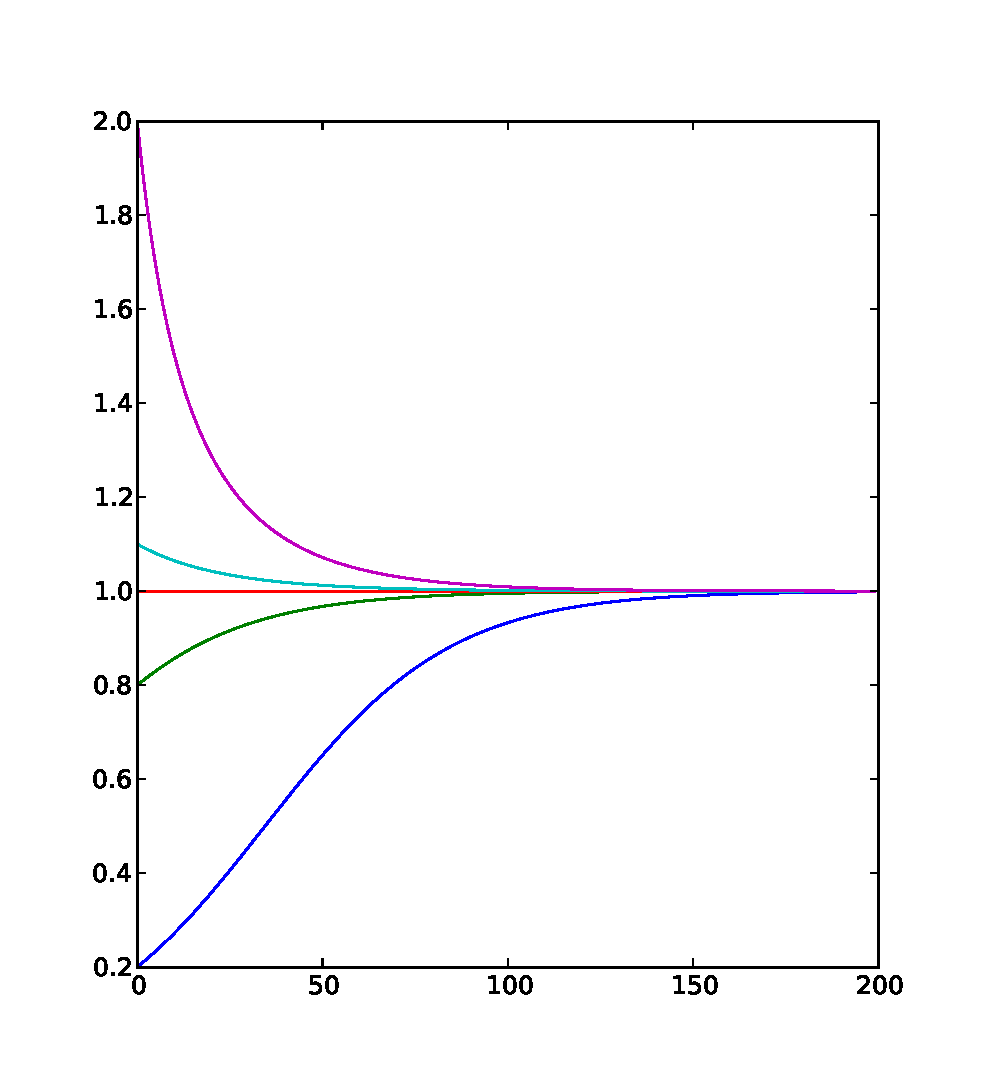
\includegraphics[width=0.75\textwidth]{logistic_diffeq_mu4_varyingx0}
    % for x in (2.0, 1.1, 1.0, 0.8, 0.3):
    %   res = rk4_1D(logistic, x, 2.0, 0.01, (4))
    %   plot(sp.linspace(0,2,201), res)
    % xlim([0,2]); ylim([0,2.01]); xticks(fontsize=24); yticks(fontsize=24)
    % xlabel(r't (time)', fontsize=26); ylabel(r'x(t)', fontsize=26)
  \end{center}
  \caption{
    Plot of equation \pref{eqn:ldesoln} with $\mu = 4$ and various initial values. 
  Regardless of the initial value, $x(t)$ converges to $1$.
}
  \label{fig:lde1}
\end{figure}
We first study the exact solution \pref{eqn:ldesoln}.
If $\mu > 0$, then $e^{\mu t} \to \infty$ as $t \to \infty$, so regardless of the initial value, $x(t)$ converges to the stable state, $x = 1$ (Figure~\ref{fig:lde1}).
%
When $\mu$ is larger, the solution curve converges faster to the stable state (Figure~\ref{fig:lde2}).
As long as $\mu > 0$, however, the asymptotic behavior of the solution does not change.
\begin{figure}[h]
  \begin{center}
    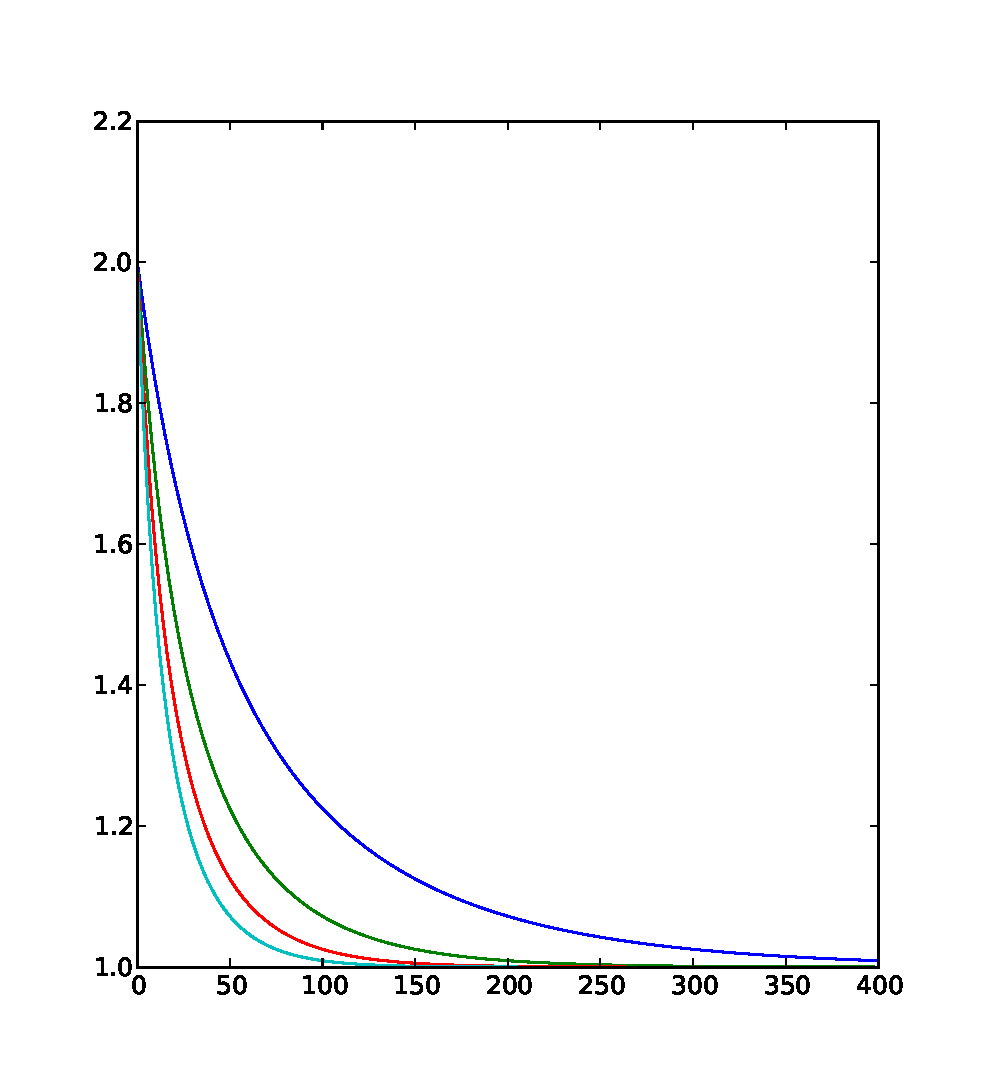
\includegraphics[width=0.75\textwidth]{logistic_diffeq_mu1234_x2}
    % for mu in (1,2,3,4):
    %   res = rk4_1D(logistic, 2.0, 5.0, 0.01, (mu))
    %   plot(sp.linspace(0,5,501), res)
    % xlim([0,5]); ylim([0.99,2.01]); xticks(fontsize=24); yticks(fontsize=24)
    % xlabel(r't (time)', fontsize=26); ylabel(r'x(t)', fontsize=26)
  \end{center}
  \caption{
    Plot of equation \pref{eqn:ldesoln} with $x_0 = 2$ and various $\mu$ ($\mu = 1,2,3,4$).
    As $\mu$ increases, $x(t)$ converges to $1$ faster.
  }
  \label{fig:lde2}
\end{figure}

Next, we study the solution of the discretized model \pref{eqn:logisticsoln} in the same manner.
For $\mu = 1$, solution curves exhibit similar behaviors as the exact solution (Figure~\ref{fig:logistic1-2}).
The stable state has changed to $x = 0$, but for any initial value, the solution curve converges to the stable state.
When $\mu = 2$, the stable state changes to $x = 0.5$.
Thus, we see that \pref{eqn:logisticsoln} does not behave in the exact same manner as \pref{eqn:ldesoln} does.
%\begin{minipage}[t]{0.5\linewidth} <- I could use this.
\begin{figure}[p]
    \centering
    \includegraphics[width=0.75\textwidth]{logistic_map_mu1_varyingx0}
    \includegraphics[width=0.75\textwidth]{logistic_map_mu2_varyingx0}
    % for x in (0.8,0.6,0.4,0.2):
    %   res = IterateList(f, x, 25, (0.25))
    %   plot(res,'o-')
    % xticks(fontsize=24); yticks(fontsize=24)
    % xlabel(r't (time)', fontsize=26); ylabel(r'x(t)', fontsize=26)
    \caption{
      Plot of Equation~\pref{eqn:logisticsoln} for 25 iterations with $\mu = 1$ (top) and $\mu = 2$ (bottom).
      Initial values are $x_0 = 0.2, 0.4, 0.6, 0.8$.
    }
    \label{fig:logistic1-2}
\end{figure}
\begin{figure}[p]
    \centering
    \includegraphics[width=0.75\textwidth]{logistic_map_mu3_varyingx0}
    \includegraphics[width=0.75\textwidth]{logistic_map_mu3_periodic}
    \caption{
      Plot of equation \pref{eqn:logisticsoln} with $\mu = 3$ for 25 (top) and 100 (bottom) iterations.
      Initial values are $x_0 = 0.2, 0.4, 0.6, 0.8$.
    }
    \label{fig:logistic3}
\end{figure}
%%%
\begin{figure}[p]
  \centering
  \includegraphics[width=0.75\textwidth]{logistic_map_mu4_varyingx0}
  \includegraphics[width=0.75\textwidth]{logistic_map_mu4_chaos}
  \caption{
    Plot of equation \pref{eqn:logisticsoln} with $\mu = 4$ for 25 (top) and 100 (bottom) iterations.
    Initial values are $x_0 = 0.2, 0.4, 0.6, 0.8$.
  }
  \label{fig:logistic4}
\end{figure}
%%%
For higher values of $\mu$, the contrast between the two solutions is even more conspicuous.
When $\mu = 3$, the dynamics is almost periodic, but not quite so (Figure~\ref{fig:logistic3}).
The dynamics for $\mu = 4$ is wildly different (Figure~\ref{fig:logistic4}).
Every solution curve moves between 0 and 1, and does not settle down to a periodic behavior.
Moreover, it seems that the solution curves are not even asymptotically periodic.
One might think that this is just a transient behavior, and the solution curves will converge to some values, or at least to some periodic behaviors if we wait long enough.
However, even after 200 or 500 iterations, the logistic map keeps behaving in the same manner (Figure~\ref{fig:chaotic_map}).
This is chaotic.
\begin{figure}[p]
  \centering
  \includegraphics[width=0.75\textwidth]{logistic_map_mu4_x02_200itr}
  \includegraphics[width=0.75\textwidth]{logistic_map_mu4_x02_500itr}
  \caption{
    $\mu = 4$. Initial value $x_0 = 0.2$.
    Top: 200 iterations. Bottom: 500 iterations.
  }
  \label{fig:chaotic_map}
\end{figure}
%%%

This kind of complex behavior arises from the logistic map, one of \textit{the simplest} non-linear equations.
The logistic map for $\mu = 4$ is also known to exhibit \textit{sensitive dependence on initial conditions}, or sensitivity for short.
\index{sensitive dependence on initial conditions}
Sensitivity is considered to be a condition that causes the complicated dynamics of the logistic map.
%Also, we will eventually identify the term ``a chaotic map'' with a mapping that exhibits sensitivity.
To see how sensitivity may bring about complex dynamics, consider the orbits of $x_0 = 0.2$ and a nearby point $y_0 = 0.2 + \epsilon$, where $\epsilon$ is a small positive real number.
Since the two orbits start out close, they remain in the vicinity of each other initially.
However, the two orbits eventually separate from each other, and the distance between them keep growing (Figure~\ref{fig:logistic_sensitivity}).
Thus, a minuscule change in the initial value causes a significant difference in the orbit.
This is not the end of the story.
After the distance between the two reached its maximum, they come closer and closer again, and repeat this process in an aperiodic manner.
\begin{figure}[p]
  \centering
  \includegraphics[width=0.75\textwidth]{logistic_map_sensitivity_x02_mu4}
  %eps = sp.finfo('float').eps
  %plot(IterateList(f, 0.2, 100, (1.0)), 'o-', markersize=8); plot(IterateList(f, 0.2+eps, 100, (1.0)), '>:', markersize=9)
  \includegraphics[width=0.75\textwidth]{logistic_map_sensitivity_x02_mu4_dist}
  % plot(sp.absolute(IterateList(f, 0.2, 100, (1.0)) - IterateList(f, 0.2+eps, 100, (1.0))))
  \caption{
    $\mu = 4$. 100 iterations.
    Initial values: $x_0 = 0.2$ and $y_0 = 0.2 + \epsilon$, where $\epsilon$ is on the order of $10^{-16}$.
    The orbit of $x_0$ is plotted with dashed lines and triangular points.
    The orbit of $y_0$ is plotted with solid lines and circular points.
    The top figure shows the two orbits, and the bottom shows the evolution of distance between them.
  }
  \label{fig:logistic_sensitivity}
\end{figure}
%%%

%In general, we can make a correspondence between continuous and discrete models
%\begin{equation}
% \begin{aligned}
%  \frac{dx(t)}{dt} = G(x(t)) &\quad\mbox{(Continuous)} \\
%  x(t + 1) = F(x(t)) &\quad\mbox{(Discrete)}
%\end{aligned}
%  \label{eqn:intro2}
%\end{equation}
%by regarding the discrete model as an approximation of the continuous model.
%%We can also make the connection by seeing the continuous model as a discrete model where each time step is infinitesimally small.
%The following approximation makes the previous statements more precise:
%\begin{equation*}
%  \frac{dx(t)}{dt} \approx \frac{x(t_0 + (n+1)\Delta t) - x(t_0 + n \Delta t)}{\Delta t}.
%\end{equation*}
%As a result of this approximation, we obtain
%\begin{equation*}
%  F(x(n)) \approx x(n) + \Delta t \cdot G(x(n)).
%\end{equation*}

As it turns out, the logistic map is chaotic in all of the four definitions that we will see.
The logistic map has other interesting properties, as well.
Expositions on the logistic map can be found in many sources.
See \citep{may1, may2, devaney}, for example.
%%%


\bibliographystyle{../../bibliography/pjgsm}
\bibliography{../../bibliography/thesis}

\end{document}
